\begin{figure}

\centering

\begin{tikzpicture}

% Axes
\draw [->, thick] ( -1, 0 ) -- ++( 9, 0 );
\draw [->, thick] ( 0, -1 ) -- ++( 0, 7 );

% Regimes
\draw [gray] ( 0, 2 ) -- ++( 2, -2 );
\draw [gray] ( 1, 1 ) -- ++( 6, 0 );
\draw [gray, dashed] ( 1, 1 ) -- ++( 4, 4 );
\draw [gray] ( 1, 1 ) -- ++( 6, 2 );
\draw [gray] ( 0, 2 ) -- ++( 6, 2 );

% Labels
\node at ( 0.5, 0.5 ) {\textcolor{gray}{I}};
\node at ( 4.5, 0.5 ) {\textcolor{gray}{II}};
\node at ( 4.5, 1.5 ) {\textcolor{gray}{III}};
\node at ( 3.5, 2.5 ) {\textcolor{gray}{IV}};
\node at ( 1.5, 3.5 ) {\textcolor{gray}{V}};

% Operating points
\draw [fill = red, draw = red] ( 2.5, 1.25 ) circle ( 0.1 );
\draw [->, red] ( 2.5, 1.25 ) -- ++( 0.2, -0.45 );
\draw [red, dashed] ( 2.75, 0.75 ) circle ( 0.1 );

\foreach \x in { 0, ..., 5 }
  \node at ( \x + 1, 0 ) [below] {\textcolor{gray}{\(10^\x\)}};
\foreach \y in { 0, ..., 4 }
  \node at ( 0, \y + 1 ) [left] {\textcolor{gray}{\(10^\y\)}};

\node at ( 3.5, -0.75 ) [below] {\(\dfrac{ L }{ \delta_f }\)};
\node at ( -0.75, 3.5 ) [left] {\(\dfrac{ u }{ S_L }\)};

\node at ( 7, 1 ) [right] {\textcolor{gray}{\(S_L = u\)}};
\node at ( 7, 3 ) [right] {\textcolor{gray}{\(Ka = 1\)}};
\node at ( 6, 4 ) [right] {\textcolor{gray}{\(Ka = 100\)}};
\node at ( 5, 5 ) [above] {\textcolor{gray}{\(Da = 1\)}};

\end{tikzpicture}

\caption[Borghi diagram]{The schematic above is a reproduction of the Borghi diagram from Figure \ref{fig:borghiDiagram}. The response of an operating point to increasing preheat temperature is schematically illustrated. If the initial operating point was in the corrugated flame regime, it would tend towards the laminar flame regime as the flame speed increases and the flame thickness slightly decreases.}

\label{fig:temperatureBorghiDiagram}

\end{figure}

